\documentclass{article}
    \usepackage{amssymb}
    \usepackage[utf8]{inputenc}
    \usepackage[russian]{babel}
    \usepackage[left=2cm,right=2cm,
        top=2cm,bottom=2cm,bindingoffset=0cm]{geometry}
    \usepackage{hyperref}
    \hypersetup{
        colorlinks=true,
        linkcolor=blue,
        filecolor=magenta,      
        urlcolor=cyan,
    }
  \usepackage{graphicx}
  \graphicspath{{pictures/}}
  \DeclareGraphicsExtensions{.pdf,.png,.jpg}

\begin{document}
\begin{center}{\hugeОтчет по курсовой работе за неделю\\}\end{center}
Дата: 5.11.2020\\
Научные руководители: Герасимов С.В., Мещеряков А.В.\\
Студент: Немешаева Алиса\\
Курс: 4\\

\renewcommand{\labelitemi}{$\blacksquare$}
\renewcommand\labelitemii{$\square$}
\begin{enumerate}
    \item На прошлой неделе было начато обучение модели только на тех областях неба, что содержат 
        в себе данные скоплений ACT. Результаты не изменились: отклик для каталогов ACT всё ещё 
        низкий. Это может быть связяно с тем, что не все скопления ACT можно обнаружить в данных 
        Planck. Поэтому часть каталога ACT была "обрезана" по параметрам M500 и z, чтобы обучить 
        новую модель и проверить эту гипотезу.\\
    \begin{figure}[h]
        \center{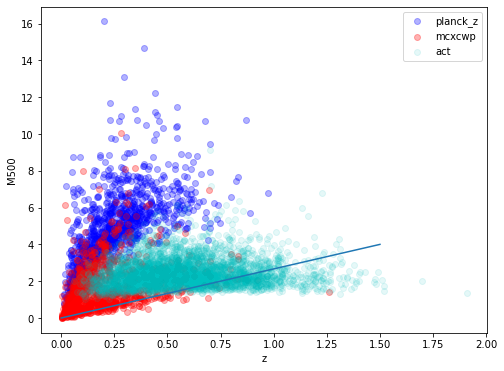
\includegraphics[width=0.6\linewidth]{before_cut}}
        \caption{Распределение скоплений каталогов planck\_z, mcxcwp, act по параметрам z и M500}
    \end{figure}
    \begin{figure}[h]
        \center{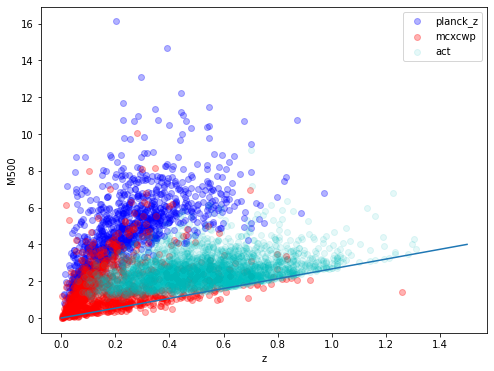
\includegraphics[width=0.6\linewidth]{after_cut}}
        \caption{Распределение скоплений каталогов planck\_z, mcxcwp, act по параметрам z и M500
            после отсечения части каталога act}
    \end{figure}

    \item Из получившихся моделей были выбраны две эпохи: 10 и 14, и на основе этих моделей были 
        созданы два каталога со следующими результатами:\\
    \begin{figure}[h]
        \center{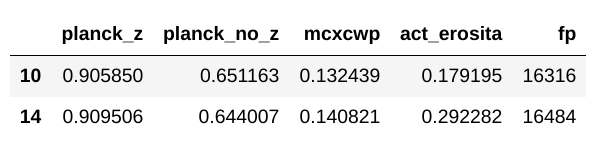
\includegraphics[width=0.6\linewidth]{table}}
        \caption{Recall и fp по новым каталогам, каталог act\_erosita - обрезанная версия каталога 
        act/}
    \end{figure}


\end{enumerate}

Отчет согласован с научным руководителем.\\
Общее количество строк кода за эту неделю: 202\\
\hyperlink{https://github.com/rt2122/data-segmentation-2}{Репозиторий}\\ 
\end{document}
